% pi-monitor-light --- Technical Note
% Build:
%   pdflatex pi-monitor-light.tex      (run twice for TOC/xrefs)
% Toolchain:
%   texlive-latex-recommended  texlive-fonts-recommended  texlive-pictures
%
% Notes:
%   - Single-file build, no biber/bibtex (uses thebibliography).
%   - No exotic fonts; ships fine on Debian/Ubuntu TeX Live 2022+.

\documentclass[11pt,a4paper]{article}

% ---------- geometry & typography ----------
\usepackage[a4paper,top=1in,bottom=1.1in,left=1.1in,right=1.1in,headheight=22pt]{geometry}
\usepackage[T1]{fontenc}
\usepackage[utf8]{inputenc}
\usepackage{lmodern}
\usepackage{mathpazo}                 % Palatino-clone body + math
\usepackage[scaled=0.92]{helvet}      % Helvetica for sans (titles)
\usepackage[scaled=0.85]{beramono}    % Bera Mono for code (compact)
\renewcommand{\familydefault}{\rmdefault}
\usepackage{microtype}
\usepackage{parskip}                  % blank-line paragraphs, no first-line indent
\usepackage{setspace}
\setstretch{1.04}

% ---------- layout helpers ----------
\usepackage{fancyhdr}
\usepackage{titlesec}
\usepackage{enumitem}
\setlist{topsep=2pt,itemsep=2pt,parsep=0pt,leftmargin=*}
\usepackage{booktabs}
\usepackage{array}
\usepackage{caption}
\captionsetup{font=small,labelfont={bf,sf},labelsep=period,format=plain}
\usepackage[hidelinks,colorlinks=true,linkcolor=black,urlcolor=blue!55!black,citecolor=blue!55!black]{hyperref}
\usepackage{url}
\usepackage{xcolor}
\definecolor{accent}{HTML}{1F4E79}
\definecolor{rule}{HTML}{8A8A8A}
\definecolor{codebg}{HTML}{F7F7F2}

% ---------- listings ----------
\usepackage{listings}
\lstdefinestyle{tn}{
  basicstyle=\ttfamily\footnotesize,
  keywordstyle=\bfseries\color{accent},
  commentstyle=\itshape\color{black!55},
  stringstyle=\color{accent!80!black},
  breaklines=true,
  columns=fullflexible,
  keepspaces=true,
  frame=single,
  framerule=0.3pt,
  rulecolor=\color{rule!60},
  backgroundcolor=\color{codebg},
  xleftmargin=6pt,
  xrightmargin=6pt,
  framexleftmargin=2pt,
  framexrightmargin=2pt,
  framextopmargin=3pt,
  framexbottommargin=3pt,
  aboveskip=8pt,
  belowskip=4pt,
  showstringspaces=false,
  literate={Ä}{{\"A}}1 {Ö}{{\"O}}1 {Ü}{{\"U}}1 {ä}{{\"a}}1 {ö}{{\"o}}1 {ü}{{\"u}}1,
}
\lstset{style=tn}
\lstdefinelanguage{systemd}{
  morekeywords={Description,After,BindsTo,ConditionPathExists,Type,User,Group,UMask,
    RuntimeDirectory,EnvironmentFile,ExecStartPre,ExecStart,ExecStopPost,
    Restart,RestartSec,Nice,ProtectSystem,ProtectHome,ReadWritePaths,
    PrivateTmp,NoNewPrivileges,StandardOutput,StandardError,WantedBy},
  morecomment=[l]{\#},
  sensitive=true,
}
\lstdefinelanguage{udevrules}{
  morekeywords={SUBSYSTEM,KERNEL,ACTION,TAG,ENV,SUBSYSTEMS,ATTRS},
  sensitive=true,
}

% ---------- TikZ ----------
\usepackage{tikz}
\usetikzlibrary{positioning,arrows.meta,shapes.geometric,backgrounds,fit,calc}

% ---------- title styling ----------
\titleformat{\section}
  {\sffamily\large\bfseries\color{accent}}
  {\thesection.}{0.6em}{}
\titleformat{\subsection}
  {\sffamily\normalsize\bfseries}
  {\thesubsection}{0.6em}{}
\titlespacing*{\section}{0pt}{14pt}{4pt}
\titlespacing*{\subsection}{0pt}{8pt}{2pt}

% ---------- header / footer ----------
\pagestyle{fancy}
\fancyhf{}
\fancyhead[L]{\sffamily\footnotesize pi-monitor-light}
\fancyhead[R]{\sffamily\footnotesize Technical Note}
\fancyfoot[C]{\sffamily\footnotesize \thepage}
\renewcommand{\headrulewidth}{0.3pt}
\renewcommand{\headrule}{\hbox to\headwidth{\color{rule!60}\leaders\hrule height \headrulewidth\hfill}}

% ---------- title block (in-page, not separate title page) ----------
\title{\vspace{-1.4cm}
  {\sffamily\bfseries\color{accent}\Large pi-monitor-light}\\[2pt]
  {\sffamily\large A power-budgeted, SSH-only UART monitor and STM32 flashing station}}
\author{\sffamily\normalsize Patrik Drazic\\[1pt]
        \small\href{https://github.com/paky12}{\nolinkurl{github.com/paky12}}\\[2pt]
        \small\textit{Technical Note}}
\date{\sffamily\small April 2026}

% ---------- abstract box ----------
\renewcommand{\abstractname}{\sffamily\normalsize\color{accent}Abstract}

\begin{document}
\maketitle
\thispagestyle{fancy}

\begin{abstract}\noindent\small
\textit{pi-monitor-light} is a single-board headless tool for embedded
firmware development: it logs up to four UART streams continuously,
flashes STM32 firmware over ST-Link, and is reachable from anywhere
on Earth over an SSH-only workflow. The implementation deliberately
uses only shell scripts, \texttt{systemd}, and \texttt{udev} --- no
Python, no web framework --- so that idle CPU is essentially zero and
the entire station fits within a 2.3\,W power envelope on a Raspberry
Pi Zero 2 W. This note documents the motivation, hardware topology,
software architecture, power budget, and design decisions behind a
deliberate \emph{build down} from a heavier prototype.
\end{abstract}

{\small
\setcounter{tocdepth}{1}
\renewcommand{\contentsname}{\sffamily\normalsize\color{accent}Contents}
\tableofcontents
}

\vspace{6pt}\hrule height 0.3pt\vspace{6pt}

% =============================================================
\section{Motivation}
% =============================================================

A prior version of this tool, \texttt{pi-monitor}, was a FastAPI web
application running on a Raspberry Pi 4 that exposed a browser UI for
dual-pane UART monitoring and OpenOCD flashing. It worked, but two
constraints made it the wrong shape for the actual deployment.

\textbf{Power.} The target deployment shares a 24\,V\,/\,0.2\,A rail
(4.8\,W total) with the rest of a custom carrier PCB. A Pi 4--class
board idling at $\sim$3\,W consumes most of that budget before any
peripherals are attached. A Pi Zero 2 W idles at well under 1\,W,
leaving room for the ST-Link and the FTDIs.

\textbf{Workflow.} The browser UI duplicated functionality that is
already cleaner over SSH: \texttt{tmux} for pane management,
\texttt{scp} for firmware transfer, \texttt{journalctl -f} for live
logs. The Python\,/\,FastAPI\,/\,SSE stack added a permanent $\sim$50\,MB
resident footprint and a userspace polling loop per pane to deliver a
UI that, in practice, was no longer needed.

The redesign target therefore was: same capabilities; total board
power $\leq$\,2.3\,W on a Pi Zero 2 W; no userspace polling; reachable
from anywhere on Earth without a public IP.

% =============================================================
\section{System overview}
% =============================================================

Figure \ref{fig:topology} shows the deployed station. The operator's
laptop joins the same Tailscale tailnet as the Pi, then SSHs to it by
its tailnet hostname; the Pi never needs an inbound public IP. On
the Pi, four small CLI wrappers (\texttt{sl-monitor}, \texttt{sl-attach},
\texttt{sl-flash}, \texttt{sl-status}) drive a \texttt{systemd}
template unit per UART, with USB hot-plug events bridged into systemd
by a \texttt{udev} rule. The data path itself is a kernel \texttt{cat}
on the tty device, piped through \texttt{ts} for timestamping and
\texttt{tee} for journaling --- no userspace polling loop.

\begin{figure}[!h]
\centering
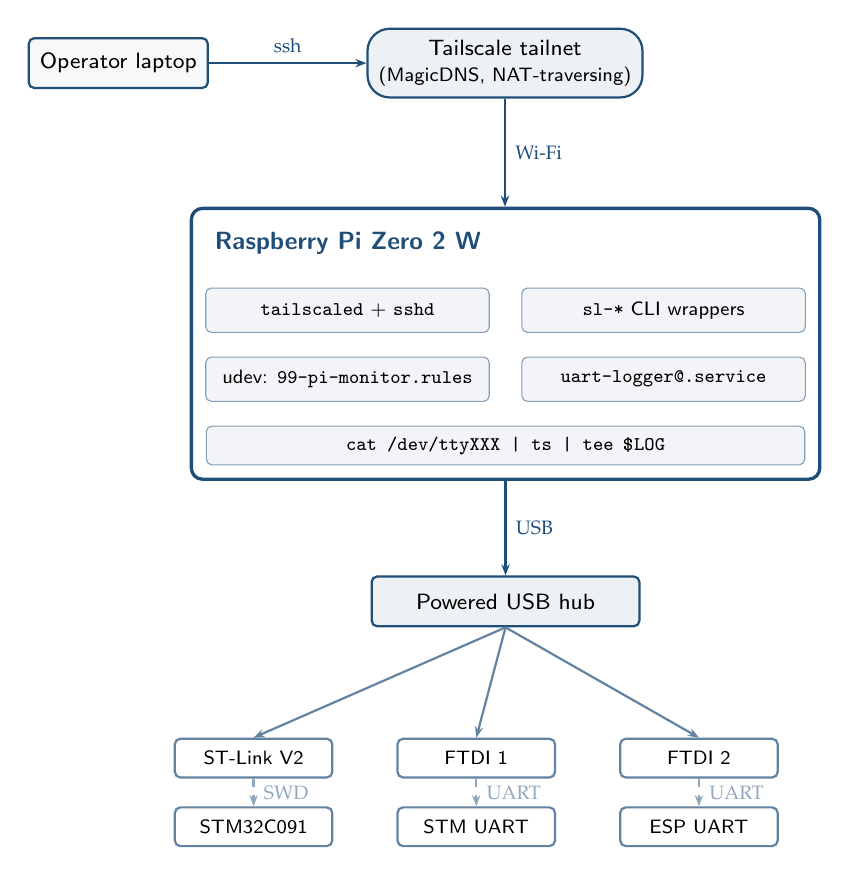
\begin{tikzpicture}[
  font=\sffamily\footnotesize,
  >={Stealth[length=4pt]},
  every node/.style={align=center},
  box/.style={draw=accent,thick,rounded corners=2pt,minimum height=18pt,
              minimum width=22mm,fill=accent!4,inner sep=4pt},
  cloud/.style={draw=accent,thick,rounded corners=8pt,fill=accent!8,
              inner sep=4pt,minimum height=18pt,minimum width=32mm},
  hub/.style={draw=accent,thick,rounded corners=2pt,minimum height=18pt,
              fill=accent!8,inner sep=3pt,minimum width=34mm},
  pi/.style={draw=accent,very thick,rounded corners=4pt},
  sub/.style={draw=accent!55,thin,rounded corners=2pt,fill=accent!6,
              minimum height=16pt,inner sep=3pt,minimum width=36mm,
              font=\sffamily\scriptsize},
  subwide/.style={sub,minimum width=76mm,minimum height=14pt},
  device/.style={draw=accent!70,thick,rounded corners=2pt,
              fill=white,minimum width=20mm,minimum height=14pt,
              inner sep=2pt,font=\sffamily\scriptsize},
]

% --- top row: laptop, cloud
\node[box] (laptop) {Operator laptop};
\node[cloud,right=20mm of laptop] (ts)
   {Tailscale tailnet\\\scriptsize(MagicDNS, NAT-traversing)};

% --- Pi internals: 2x2 grid + wide data row, drawn FIRST,
%     then a fit container is wrapped around them.
\node[sub,below=24mm of ts,xshift=-20mm]
     (svc1) {\texttt{tailscaled} + \texttt{sshd}};
\node[sub,right=4mm of svc1]
     (svc2) {\texttt{sl-*} CLI wrappers};
\node[sub,below=3mm of svc1.south west,anchor=north west]
     (sys1) {udev: \texttt{99-pi-monitor.rules}};
\node[sub,right=4mm of sys1]
     (sys2) {\texttt{uart-logger@.service}};
\coordinate (gridmid) at ($(sys1.south)!0.5!(sys2.south)$);
\node[subwide,below=3mm of gridmid,anchor=north]
     (data) {\texttt{cat /dev/ttyXXX | ts | tee \$LOG}};

% Title above the grid (will be enclosed by the fit container)
\node[font=\sffamily\small\bfseries\color{accent},
      above=3mm of svc1.north west,anchor=south west]
     (pititle) {Raspberry Pi Zero 2 W};

% Container wraps the title + all internals
\node[pi,fit=(pititle)(svc1)(svc2)(sys1)(sys2)(data),inner sep=5pt] (pi) {};

% --- USB hub well below pi
\node[hub,below=12mm of pi.south] (hub) {Powered USB hub};

% --- target row
\node[device,below=14mm of hub.south,xshift=-32mm] (stl)   {ST-Link V2};
\node[device,right=8mm of stl]                       (ftdi1) {FTDI 1};
\node[device,right=8mm of ftdi1]                     (ftdi2) {FTDI 2};
\node[device,below=10pt of stl]                      (stm)   {STM32C091};
\node[device,below=10pt of ftdi1]                    (mcu1)  {STM UART};
\node[device,below=10pt of ftdi2]                    (mcu2)  {ESP UART};

% --- arrows
\draw[->,thick,accent] (laptop) -- node[above,font=\scriptsize]{ssh} (ts);
\draw[->,thick,accent] (ts.south) -- node[right,font=\scriptsize]{Wi-Fi}
       (pi.north -| ts.south);
\draw[->,thick,accent] (pi.south) -- node[right,font=\scriptsize]{USB} (hub.north);
\draw[->,thick,accent!70] (hub.south) -- (stl.north);
\draw[->,thick,accent!70] (hub.south) -- (ftdi1.north);
\draw[->,thick,accent!70] (hub.south) -- (ftdi2.north);
\draw[->,thick,accent!50,dashed] (stl)   -- node[right,font=\scriptsize]{SWD}  (stm);
\draw[->,thick,accent!50,dashed] (ftdi1) -- node[right,font=\scriptsize]{UART} (mcu1);
\draw[->,thick,accent!50,dashed] (ftdi2) -- node[right,font=\scriptsize]{UART} (mcu2);

\end{tikzpicture}
\caption{End-to-end topology. Solid lines are TCP/USB; dashed lines are
the SWD/UART pin connections to the device under test. The Pi has no
public IP; remote reachability comes from Tailscale.}
\label{fig:topology}
\end{figure}

% =============================================================
\section{Hardware}
% =============================================================

The station is a small daisy-chain of off-the-shelf parts. The
custom carrier PCB supplies 5\,V to the Pi via the GPIO header; no
SD-card swap, HDMI output, or display is used in production.

\begin{table}[!h]
\centering\small
\renewcommand{\arraystretch}{1.15}
\begin{tabular}{@{} l l r @{}}
\toprule
\textbf{Component} & \textbf{Role} & \textbf{Idle draw} \\
\midrule
Raspberry Pi Zero 2 W              & SoC + Wi-Fi              & 0.5--0.7\,W \\
ST-Link V2                         & STM32 SWD programmer     & 0.10--0.15\,W \\
FTDI TTL-232R-3V3 $\times N$ ($N$=1..4) & Per-port UART tap   & $\sim$0.05--0.08\,W each \\
Powered USB hub                    & ST-Link + FTDI fan-out   & 0.10--0.20\,W \\
24\,V $\rightarrow$ 5\,V buck      & Carrier-PCB power conditioning & --- \\
\bottomrule
\end{tabular}
\caption{Bill of materials. The Pi Zero 2 W's single micro-USB-OTG
port forces the use of a powered hub; this is the only ``required''
peripheral beyond the targets themselves.}
\label{tab:bom}
\end{table}

% =============================================================
\section{Software architecture}
% =============================================================

\subsection{Data path: zero userspace polling}

The core observation is that ``log a UART to disk'' is not a problem
that needs userspace logic --- the kernel already has the relevant
primitives. The whole data path is one shell pipeline (Listing
\ref{lst:execstart}, line 6): \texttt{cat} blocks in the kernel on a
serial \texttt{read()} until bytes arrive (zero CPU when idle),
\texttt{ts} from \texttt{moreutils} prepends a per-line timestamp,
and \texttt{tee -a} writes to the log file while forwarding to
\texttt{systemd}'s journal. There is no userspace polling loop
anywhere in the data path.

\subsection{Lifecycle: udev + systemd handshake}

The non-trivial part is making this resilient across USB hot-plug and
across reboots. The mechanism is a two-sided handshake between
\texttt{udev} and a \texttt{systemd} template unit
(\texttt{uart-logger@.service}):

\begin{itemize}
  \item \textbf{Start} on USB \texttt{add}: a udev rule
    (Listing \ref{lst:udev}) tags the new \texttt{ttyUSB*} or
    \texttt{ttyACM*} device with \texttt{TAG+="systemd"} and
    \texttt{ENV\{SYSTEMD\_WANTS\}+="uart-logger@\%k.service"},
    which causes \texttt{systemd} to instantiate the per-device unit.
  \item \textbf{Stop} on USB \texttt{remove}: \texttt{BindsTo=dev-\%i.device}
    in the unit makes \texttt{systemd} follow the device unit's
    lifecycle. Removal stops the logger and triggers
    \texttt{ExecStopPost} to write a session-end marker plus
    duration.
  \item \textbf{Restart} on transient failure: \texttt{Restart=on-failure}
    handles the case where the device is still present but the
    pipeline died (e.g.\ EIO). Importantly, this does \emph{not} fire
    on \texttt{BindsTo}-driven stops --- those are systemd-driven and
    are explicitly excluded by \texttt{Restart=}\,\cite{systemd-service}.
    The udev re-fire on the next \texttt{add} is the recovery path.
\end{itemize}

\begin{lstlisting}[language=udevrules,caption={\texttt{udev} rule
that bridges USB hot-plug into systemd. Both \texttt{ttyUSB*} (FTDI,
CP210x) and \texttt{ttyACM*} (CDC-ACM) are matched.},label={lst:udev}]
SUBSYSTEM=="tty", KERNEL=="ttyUSB[0-9]*", ACTION=="add", \
  TAG+="systemd", ENV{SYSTEMD_WANTS}+="uart-logger@%k.service"

SUBSYSTEM=="tty", KERNEL=="ttyACM[0-9]*", ACTION=="add", \
  TAG+="systemd", ENV{SYSTEMD_WANTS}+="uart-logger@%k.service"
\end{lstlisting}

The unit (Listing \ref{lst:execstart}) runs as a dedicated system user
\texttt{pi-monitor} and is sandboxed by \texttt{ProtectSystem=strict},
\texttt{ProtectHome=yes}, \texttt{NoNewPrivileges=yes}, with
\texttt{ReadWritePaths=} restricted to the log and runtime directories.

\begin{lstlisting}[language=systemd,caption={Excerpt of the systemd
template unit. The \texttt{ExecStart} pipeline is the entire data
path; everything else is policy. \texttt{ConditionPathExists} silently
skips the unit for ports not present in \texttt{ports.conf}, avoiding
``failed unit'' clutter for irrelevant USB-serial devices.},label={lst:execstart}]
[Unit]
Description=UART logger on /dev/%i
After=dev-%i.device
BindsTo=dev-%i.device
ConditionPathExists=/etc/pi-monitor-light/ports.conf.env-%i

[Service]
User=pi-monitor
EnvironmentFile=/etc/pi-monitor-light/ports.conf.env-%i
ExecStartPre=/usr/bin/stty -F /dev/%i ${BAUD} raw -echo -crtscts
ExecStart=/bin/bash -ec 'set -o pipefail; \
  LOG="/var/log/pi-monitor/${NAME}/$(date +%%Y-%%m-%%d_%%H-%%M-%%S).log"; \
  exec /usr/bin/cat /dev/%i | /usr/bin/ts | /usr/bin/tee -a "$LOG"'
Restart=on-failure
ProtectSystem=strict
ProtectHome=yes
NoNewPrivileges=yes
\end{lstlisting}

\subsection{Operator interface}

Five thin shell wrappers expose the system to the operator.
\texttt{sl-monitor up\,|\,down\,|\,restart} enables or disables logger
units based on \texttt{ports.conf}; \texttt{sl-attach} opens a
\texttt{tmux} session with one window per active port running
\texttt{journalctl -u uart-logger@<port> -f}; \texttt{sl-flash <bin>}
flashes a firmware binary via OpenOCD, rejecting path-traversal,
non-\texttt{.bin} files, and filenames with shell-special characters
that could escape the OpenOCD Tcl \texttt{program} command. The
\texttt{ports.conf} parser enforces device-name format, name charset
(\texttt{[A-Za-z0-9\_-]+}, used as a log subdirectory name),
duplicate detection, and a trailing-comment carve-out, so the systemd
template instantiation cannot be coerced into a malformed unit name.

\subsection{Flashing toolchain}

OpenOCD is the only cross-platform open-source SWD programmer that
supports the STM32C0 series. The relevant target configuration
\texttt{tcl/target/stm32c0x.cfg} was added to OpenOCD master
\emph{after} the 0.12.0 release; consequently the Bookworm package
\cite{debian-openocd} cannot flash the STM32C091 used here. The
installer therefore builds OpenOCD from the project's GitHub mirror
\cite{openocd-mirror} during first-time setup. Build time on a Pi
Zero 2 W is approximately 30 minutes; an environment override
\texttt{OPENOCD\_JOBS=-j1} exists for the OOM case on the 512\,MB
device.

% =============================================================
\section{Power budget}
% =============================================================

The 2.3\,W ceiling derives from the carrier PCB's 24\,V\,/\,0.2\,A rail
(4.8\,W total) less the rest of the carrier's load. Table
\ref{tab:power} lists the design targets.

\begin{table}[!h]
\centering\small
\renewcommand{\arraystretch}{1.15}
\begin{tabular}{@{} l r @{}}
\toprule
\textbf{Element} & \textbf{Estimated draw} \\
\midrule
Pi Zero 2 W idle (BT off, ACT LED off, 2 of 4 cores enabled) & 0.5--0.7\,W \\
ST-Link V2 idle                                              & 0.10--0.15\,W \\
FTDI TTL-232R-3V3 $\times 2$                                 & $\sim$0.10--0.15\,W \\
Powered USB hub overhead                                     & 0.10--0.20\,W \\
\midrule
\textbf{Total idle (target)}                                 & \textbf{$\sim$1.0--1.4\,W} \\
\textbf{Total during a flash (transient peak)}               & \textbf{$\sim$1.8--2.2\,W} \\
\bottomrule
\end{tabular}
\caption{Power budget. Numbers are design targets; the authoritative
test is a USB power meter on the Pi's 5\,V rail with all peripherals
attached and a flash in progress.}
\label{tab:power}
\end{table}

The CPU-side savings come from three layered tweaks applied via
\texttt{config.txt} and \texttt{cmdline.txt}\,\cite{rpi-config}:
\textbf{(1)}~\texttt{dtoverlay=disable-bt} disables the Bluetooth
controller; \textbf{(2)}~\texttt{maxcpus=2} parks two of the four
Cortex-A53 cores --- idle is nearly identical to single-core, and
flash is faster than \texttt{maxcpus=1} without the OOM risk during
the OpenOCD build; \textbf{(3)}~ACT LED off and boot splash disabled.
Headroom against the 2.3\,W ceiling is therefore on the order of
100--500\,mW depending on flash load --- thin enough that it has to
be measured rather than computed. A documented fallback
(\texttt{maxcpus=1}, \texttt{arm\_freq=600}) exists for the case
where measured draw exceeds budget.

% =============================================================
\section{Operator workflow}
% =============================================================

Once installed (\texttt{sudo ./install.sh} on a fresh Bookworm Lite
image), the daily workflow from any device on the tailnet is:

\begin{lstlisting}[language=bash]
ssh patrik@pi-monitor
sl-attach                                    # tmux, one window per UART
scp firmware.bin pi-monitor:/var/lib/pi-monitor/firmware/
sl-flash /var/lib/pi-monitor/firmware/firmware.bin
\end{lstlisting}

Per-site Wi-Fi onboarding uses a phone hotspot with a fixed SSID as a
stable bootstrap: the Pi always knows that hotspot, joins it whenever
in range, and from that initial connection the operator adds the
local Wi-Fi via \texttt{nmcli device wifi connect}. The site
credentials persist across reboots and the phone hotspot is no longer
needed once the site is known. The \texttt{README.md} in the
repository contains the operator-facing reference for these flows.

% =============================================================
\section{Design discussion}
% =============================================================

A handful of choices visibly shaped the final system.

\paragraph{Shell + systemd over a daemon.}
A Go or Rust daemon would be roughly the same lines of code but
introduces a long-running process to maintain. \texttt{systemd}
already solves unit lifecycle, restart policy, sandboxing, log
rotation, and template instantiation. Implementing those once in
shell glue and delegating the rest avoided a class of recurring
engineering work. The 47-test \texttt{bats} suite that came out of
this is genuinely small --- the parser library is the only piece
with non-trivial logic.

\paragraph{Tailscale over SSH-on-public-IP.}
Tailscale gives transitive zero-config NAT traversal and built-in SSH
authentication via the tailnet identity \cite{tailscale-ssh}, removing
port forwarding, dynamic DNS, and per-host SSH key distribution. The
operational overhead on the Pi is a single \texttt{tailscaled}
process ($\sim$15\,MB resident, negligible idle CPU). For a tool that
travels to client sites with arbitrary Wi-Fi, this is the difference
between ``works everywhere'' and ``works on the LAN where you set it up.''

\paragraph{New log file per reconnect, not one continuous file.}
The previous \texttt{pi-monitor} version maintained one file per UI
session and inlined \texttt{--- disconnected --- / --- connected ---}
markers. The current design produces one file per
\texttt{add}-to-\texttt{remove} cycle of the device. The data is the
same; the difference is whose responsibility it is. Letting systemd
plus the filesystem be the system of record (one file per unit start)
is simpler than threading custom backoff state through a userspace
process.

\paragraph{Source-built OpenOCD with a contrib udev rule.}
A subtlety caught during review: \texttt{make install} for OpenOCD
does \emph{not} drop its \texttt{contrib/60-openocd.rules} into
\texttt{/etc/udev/rules.d/}, and without it the operator user gets
\texttt{LIBUSB\_ERROR\_ACCESS} on the ST-Link USB endpoint. The
installer copies the rule explicitly and adds the operator to
\texttt{plugdev}. This is exactly the kind of cross-task integration
issue that per-component tests cannot catch.

% =============================================================
\section{Limitations and future work}
% =============================================================

The design intentionally excludes a browser UI, live preview before
session start, command injection back to the device, and off-box log
aggregation. None of those have been needed in practice; if they
become so, the natural place to add them is a separate companion
service that consumes the existing log files rather than reshaping
the data path.

The 2.3\,W ceiling has been computed but not measured. The
authoritative test is a USB power meter on the Pi's 5\,V rail with
all peripherals attached and a flash in progress; if measured draw
exceeds 460\,mA, the documented fallback path is single-core
operation (\texttt{maxcpus=1}) and a frequency cap
(\texttt{arm\_freq=600}), which the design analysis suggests would
buy another $\sim$200--300\,mW at modest cost to flash time.

The OpenOCD master tracking is convenient now but accrues maintenance
debt: when upstream cuts a 0.13.x release with stable STM32C0
support, the installer should switch to the apt-installed package and
delete the from-source build path. The skip-check regex already
accommodates the version transition.

% =============================================================
\section*{Repository \& author}
% =============================================================

Source, design document, implementation plan, and operator README live
in the project repository under \texttt{pi-monitor-light/}. The design
document under \texttt{docs/plans/} contains the verified citations
for every systemd directive, Pi boot config option, and external
service decision used in this writeup.

\smallskip\noindent
Author: Patrik Drazic ---
\href{https://github.com/paky12}{\nolinkurl{github.com/paky12}}

% =============================================================
\begin{thebibliography}{9}\small
\bibitem{systemd-service}
systemd Project. \emph{systemd.service(5) man page --- Restart=}.
\url{https://www.freedesktop.org/software/systemd/man/latest/systemd.service.html#Restart=}

\bibitem{rpi-config}
Raspberry Pi Ltd. \emph{Raspberry Pi Documentation --- config.txt}.
\url{https://www.raspberrypi.com/documentation/computers/config_txt.html}

\bibitem{debian-openocd}
Debian Project. \emph{Package: openocd (0.12.0-1) --- Bookworm}.
\url{https://packages.debian.org/bookworm/openocd}

\bibitem{openocd-mirror}
OpenOCD Project. \emph{openocd-org/openocd --- official GitHub mirror}.
\url{https://github.com/openocd-org/openocd}

\bibitem{tailscale-ssh}
Tailscale Inc. \emph{Tailscale SSH}.
\url{https://tailscale.com/kb/1193/tailscale-ssh}

\bibitem{rpi-zero2-brief}
Raspberry Pi Ltd. \emph{Raspberry Pi Zero 2 W product brief}.
\url{https://datasheets.raspberrypi.com/rpizero2/raspberry-pi-zero-2-w-product-brief.pdf}
\end{thebibliography}

\end{document}
